\documentclass[12pt,twoside]{article}
\usepackage[dvipsnames]{xcolor}
\usepackage{tikz,graphicx,amsmath,amsfonts,amscd,amssymb,bm,cite,epsfig,epsf,url}
\usepackage[hang,flushmargin]{footmisc}
\usepackage[colorlinks=true,urlcolor=blue,citecolor=blue]{hyperref}
\usepackage{amsthm,multirow,wasysym,appendix}
\usepackage{array,subcaption} 
\usepackage{bbm}
\usepackage{pgfplots}
\usetikzlibrary{spy}
\usepgfplotslibrary{external}
\usepgfplotslibrary{fillbetween}
\usetikzlibrary{arrows,automata}
\usepackage{thmtools}
\usepackage{blkarray} 
\usepackage{textcomp}
\usepackage[left=0.8in,right=1.0in,top=1.0in,bottom=1.0in]{geometry}

\usepackage{times}
\usepackage{amsfonts}
\usepackage{amsmath}
\usepackage{latexsym}
\usepackage{color}
\usepackage{graphics}
\usepackage{enumerate}
\usepackage{amstext}
\usepackage{blkarray}
\usepackage{url}
\usepackage{epsfig}
\usepackage{bm}
\usepackage{hyperref}
\hypersetup{
    colorlinks=true,
    linkcolor=blue,
    filecolor=magenta,      
    urlcolor=blue,
}
\usepackage{textcomp}
\usepackage[left=0.8in,right=1.0in,top=1.0in,bottom=1.0in]{geometry}
\usepackage{mathtools}
\usepackage{minted}

%% Probability operators and functions
%
% \def \P{\mathrm{P}}
\def \P{\mathrm{P}}
\def \E{\mathrm{E}}
\def \Var{\mathrm{Var}}
\let\var\Var
\def \Cov {\mathrm{Cov}} \let\cov\Cov
\def \MSE {\mathrm{MSE}} \let\mse\MSE
\def \sgn {\mathrm{sgn}}
\def \R {\mathbb{R}}
\def \C {\mathbb{C}}
\def \N {\mathbb{N}}
\def \Z {\mathbb{Z}}
\def \cV {\mathcal{V}}
\def \cS {\mathcal{S}}
\DeclareMathOperator*{\argmin}{arg\,min}
\DeclareMathOperator*{\argmax}{arg\,max}
\newcommand{\red}[1]{\textcolor{red}{#1}}
\newcommand{\blue}[1]{\textcolor{blue}{#1}}
\newcommand{\green}[1]{\textcolor{ForestGreen}{ #1}}
\newcommand{\fuchsia}[1]{\textcolor{RoyalPurple}{ #1}}

%
%% Probability distributions
%
%\def \Bern    {\mathrm{Bern}}
%\def \Binom   {\mathrm{Binom}}
%\def \Exp     {\mathrm{Exp}}
%\def \Geom    {\mathrm{Geom}}
%\def \Norm    {\mathcal{N}}
%\def \Poisson {\mathrm{Poisson}}
%\def \Unif    {\mathrm {U}}
%
\newcommand{\bdb}[1]{\textcolor{red}{#1}}

\newcommand{\ml}[1]{\mathcal{ #1 } }
\newcommand{\wh}[1]{\widehat{ #1 } }
\newcommand{\wt}[1]{\widetilde{ #1 } }
\newcommand{\conj}[1]{\overline{ #1 } }
\newcommand{\rnd}[1]{\tilde{ #1 } }
\newcommand{\rv}[1]{ \rnd{ #1}  }
\newcommand{\rx}{\rnd{ x}  }
\newcommand{\ry}{\rnd{ y}  }
\newcommand{\ra}{\rnd{ a}  }
\newcommand{\rb}{\rnd{ b}  }
\newcommand{\rpc}{\widetilde{ pc}  }

\def \cnd {\, | \,}
\def \Id { I }
\def \J {\mathbf{1}\mathbf{1}^T}

\newcommand{\op}[1]{\operatorname{#1}}
\newcommand{\setdef}[2]{ := \keys{ #1 \; | \; #2 } }
\newcommand{\set}[2]{ \keys{ #1 \; | \; #2 } }
\newcommand{\sign}[1]{\op{sign}\left( #1 \right) }
\newcommand{\trace}[1]{\op{tr}\left( #1 \right) }
\newcommand{\tr}[1]{\op{tr}\left( #1 \right) }
\newcommand{\inv}[1]{\left( #1 \right)^{-1} }
\newcommand{\abs}[1]{\left| #1 \right|}
\newcommand{\sabs}[1]{| #1 |}
\newcommand{\keys}[1]{\left\{ #1 \right\}}
\newcommand{\sqbr}[1]{\left[ #1 \right]}
\newcommand{\sbrac}[1]{ ( #1 ) }
\newcommand{\brac}[1]{\left( #1 \right) }
\newcommand{\bbrac}[1]{\big( #1 \big) }
\newcommand{\Bbrac}[1]{\Big( #1 \Big)}
\newcommand{\BBbrac}[1]{\BIG( #1 \Big)}
\newcommand{\MAT}[1]{\begin{bmatrix} #1 \end{bmatrix}}
\newcommand{\sMAT}[1]{\left(\begin{smallmatrix} #1 \end{smallmatrix}\right)}
\newcommand{\sMATn}[1]{\begin{smallmatrix} #1 \end{smallmatrix}}
\newcommand{\PROD}[2]{\left \langle #1, #2\right \rangle}
\newcommand{\PRODs}[2]{\langle #1, #2 \rangle}
\newcommand{\der}[2]{\frac{\text{d}#2}{\text{d}#1}}
\newcommand{\pder}[2]{\frac{\partial#2}{\partial#1}}
\newcommand{\derTwo}[2]{\frac{\text{d}^2#2}{\text{d}#1^2}}
\newcommand{\ceil}[1]{\lceil #1 \rceil}
\newcommand{\Imag}[1]{\op{Im}\brac{ #1 }}
\newcommand{\Real}[1]{\op{Re}\brac{ #1 }}
\newcommand{\norm}[1]{\left|\left| #1 \right|\right| }
\newcommand{\norms}[1]{ \| #1 \|  }
\newcommand{\normProd}[1]{\left|\left| #1 \right|\right| _{\PROD{\cdot}{\cdot}} }
\newcommand{\normTwo}[1]{\left|\left| #1 \right|\right| _{2} }
\newcommand{\normTwos}[1]{ \| #1  \| _{2} }
\newcommand{\normZero}[1]{\left|\left| #1 \right|\right| _{0} }
\newcommand{\normTV}[1]{\left|\left| #1 \right|\right|  _{ \op{TV}  } }% _{\op{c} \ell_1} }
\newcommand{\normOne}[1]{\left|\left| #1 \right|\right| _{1} }
\newcommand{\normOnes}[1]{\| #1 \| _{1} }
\newcommand{\normOneTwo}[1]{\left|\left| #1 \right|\right| _{1,2} }
\newcommand{\normF}[1]{\left|\left| #1 \right|\right| _{\op{F}} }
\newcommand{\normLTwo}[1]{\left|\left| #1 \right|\right| _{\ml{L}_2} }
\newcommand{\normNuc}[1]{\left|\left| #1 \right|\right| _{\ast} }
\newcommand{\normOp}[1]{\left|\left| #1 \right|\right|  }
\newcommand{\normInf}[1]{\left|\left| #1 \right|\right| _{\infty}  }
\newcommand{\proj}[1]{\mathcal{P}_{#1} \, }
\newcommand{\diff}[1]{ \, \text{d}#1 }
\newcommand{\vc}[1]{\boldsymbol{\vec{#1}}}
\newcommand{\rc}[1]{\boldsymbol{#1}}
\newcommand{\vx}{\vec{x}}
\newcommand{\vy}{\vec{y}}
\newcommand{\vz}{\vec{z}}
\newcommand{\vu}{\vec{u}}
\newcommand{\vv}{\vec{v}}
\newcommand{\vb}{\vec{\beta}}
\newcommand{\va}{\vec{\alpha}}
\newcommand{\vaa}{\vec{a}}
\newcommand{\vbb}{\vec{b}}
\newcommand{\vg}{\vec{g}}
\newcommand{\vw}{\vec{w}}
\newcommand{\vh}{\vec{h}}
\newcommand{\vnu}{\vec{\nu}}
\newcommand{\rvnu}{\vc{\nu}}

\newtheorem{theorem}{Theorem}[section]
% \declaretheorem[style=plain,qed=$\square$]{theorem}
\newtheorem{corollary}[theorem]{Corollary}
\newtheorem{definition}[theorem]{Definition}
\newtheorem{lemma}[theorem]{Lemma}
\newtheorem{remark}[theorem]{Remark}
\newtheorem{algorithm}[theorem]{Algorithm}

% \theoremstyle{definition}
%\newtheorem{example}[proof]{Example}
%\declaretheorem[style=definition,qed=$\triangle$,sibling=definition]{example}
%\declaretheorem[style=definition,qed=$\bigcirc$,sibling=definition]{application}

%
%% Typographic tweaks and miscellaneous
%\newcommand{\sfrac}[2]{\mbox{\small$\displaystyle\frac{#1}{#2}$}}
%\newcommand{\suchthat}{\kern0.1em{:}\kern0.3em}
%\newcommand{\qqquad}{\kern3em}
%\newcommand{\cond}{\,|\,}
%\def\Matlab{\textsc{Matlab}}
%\newcommand{\displayskip}[1]{\abovedisplayskip #1\belowdisplayskip #1}
%\newcommand{\term}[1]{\emph{#1}}
%\renewcommand{\implies}{\;\Rightarrow\;}

% My macros

\def\Kset{\mathbb{K}}
\def\Nset{\mathbb{N}}
\def\Qset{\mathbb{Q}}
\def\Rset{\mathbb{R}}
\def\Sset{\mathbb{S}}
\def\Zset{\mathbb{Z}}
\def\squareforqed{\hbox{\rlap{$\sqcap$}$\sqcup$}}
\def\qed{\ifmmode\squareforqed\else{\unskip\nobreak\hfil
\penalty50\hskip1em\null\nobreak\hfil\squareforqed
\parfillskip=0pt\finalhyphendemerits=0\endgraf}\fi}

%\DeclareMathOperator*{\E}{\rm E}
%\DeclareMathOperator*{\argmax}{\rm argmax}
%\DeclareMathOperator*{\argmin}{\rm argmin}
%\DeclareMathOperator{\sgn}{sign}
\DeclareMathOperator{\supp}{supp}
\DeclareMathOperator{\last}{last}
%\DeclareMathOperator{\sign}{\sgn}
\DeclareMathOperator{\diag}{diag}
\providecommand{\abs}[1]{\lvert#1\rvert}
\providecommand{\norm}[1]{\lVert#1\rVert}
\def\vcdim{\textnormal{VCdim}}
\DeclareMathOperator*{\B}{\textbf{B}}

%\DeclarePairedDelimiter\ceil{\lceil}{\rceil}
%\DeclarePairedDelimiter\floor{\lfloor}{\rfloor}

\newcommand{\cX}{{\mathcal X}}
\newcommand{\cY}{{\mathcal Y}}
\newcommand{\cA}{{\mathcal A}}
\newcommand{\ignore}[1]{}
\newcommand{\bi}{\begin{itemize}}
\newcommand{\ei}{\end{itemize}}
\newcommand{\be}{\begin{enumerate}}
\newcommand{\ee}{\end{enumerate}}
\newcommand{\bd}{\begin{description}}
\newcommand{\ed}{\end{description}}
\newcommand{\h}{\widehat}
\newcommand{\e}{\epsilon}
\newcommand{\mat}[1]{{\mathbf #1}}
%\newcommand{\R}{\mat{R}}
\newcommand{\0}{\mat{0}}
\newcommand{\M}{\mat{M}}

\newcommand{\D}{\mat{D}}
\renewcommand{\r}{\mat{r}}
\newcommand{\x}{\mat{x}}
\renewcommand{\u}{\mat{u}}
\renewcommand{\v}{\mat{v}}
\newcommand{\w}{\mat{w}}
\renewcommand{\H}{\text{0}}
\newcommand{\T}{\text{1}}
%\newcommand{\set}[1]{\{#1\}}
\newcommand{\xxi}{{\boldsymbol \xi}}
\newcommand{\ssigma}{{\boldsymbol \sigma}}
\newcommand{\Alpha}{{\boldsymbol \alpha}}
\newcommand{\tts}{\tt \small}
\newcommand{\hint}{\emph{hint}}
\newcommand{\matr}[1]{\bm{#1}}     % ISO complying version
\newcommand{\vect}[1]{\bm{#1}} % vectors

%\newcommand{\Var}{\mathrm{Var}}
%\newcommand{\Cov}{\mathrm{Cov}}

% New commands
\newcommand{\SP}{\mathbf{S}_{+}^n}
\newcommand{\Proj}{\mathcal{P}_{\mathcal{S}}}
\DeclarePairedDelimiterX{\inp}[2]{\langle}{\rangle}{#1, #2}
\newtheorem{proof}{Proof}


\begin{document}

\noindent DS-GA.1013 Mathematical Tools for Data Science \\
Homework 4\\
Yves Greatti - yg390\\

\begin{enumerate}

\item (Condition number) Let $A\in \R^{n\times n}$ be invertible, and let $x_{\op{true}},y\in \R^n$
  satisfy $Ax_{\op{true}}=y$. We are interested in what happens if $y$ is perturbed additively by a vector $z\in \R^n$, i.e. if we solve 
\begin{align}
A w=y+z.
\end{align}
  \begin{enumerate}
  \item The operator norm of a matrix $M$ is equal to 
  \begin{align}
  \norm{M} := \max_{\normTwo{v} = 1} \normTwo{Mv},
  \end{align}  
  which we know is equal to the maximum singular value. What is the operator norm of $A^{-1}$?\\
  
  \medskip
  First A is invertible if and only if $A x = 0$ admits the only solution $x=0$ (if not $Ker(A) \neq {0}$ and A is not full row rank). 
  $A$ being symmetric by the spectral theorem, we have $A=U S U^T$ and we can compute an SVD of A by $A=U |S| U^T$.
  Then 0 cannot be an eigenvalue or a singular value, and A has only positive singular values, let $s_1 \ge \ldots \ge s_n > 0$, these singular values.
  A is invertible so $A A^{-1} = I$, let the SVD of A be $U S V^T$ then $A A^{-1} = U S V^T A^{-1} = I$.
  $U, V$ being orthonormal matrices, and multiplying on both sides by $U^T, S^{-1}, V$, we have $A^{-1} =  V S^{-1} U^T$.
  Therefore the singular values of $A^{-1}$ are $\frac{1}{s_n} \ge \ldots \ge \frac{1}{s_1}$ thus $\norm{A^{-1}} =  \max_{\normTwo{v} = 1} \normTwo{A^{-1}v} = \frac{1}{s_n}$.
  \medskip
    
  \item Prove that $\|w-x_{\op{true}}\|_2 \leq \|z\|_2/s_n$, where
    $s_j$ denotes the $j$th singular value of $A$. \\
    
  \begin{proof}
  	$A (w - x_{\op{true}}) = A w - A x_{\op{true}} = y + z - y = z$. Hence
	$$ \| A ^{-1} A (w - x_{\op{true}}) \|_2 = \| w - x_{\op{true}} \|_2 = \| A^{-1} z \|_2 $$
	$L_2$ norm being consistent $\| A^{-1} z \|_2 \| \le \norm{A^{-1}} \| z \|_2 \le \|z\|_2/s_n$.

  \end{proof}
  
  \item If $x_{\op{true}}\neq 0$ prove that
    $$\frac{\|w-x_{\op{true}}\|_2}{\|x_{\op{true}}\|_2} \leq
    \kappa(A)\frac{\|z\|_2}{\|y\|_2}.$$
    Here $\kappa(A):=s_1/s_n$ is called the \textit{condition
    number} of $A$. \\

  \medskip  
  Similarly to part (b), we have 
	
	\begin{align*}
		\| A ^{-1}  A x_{\op{true}} \|_2 	&=	\|  A ^{-1} y \|_2 \\
				\|x_{\op{true}} \|_2	&=  	\|  A ^{-1} y \|_2 \\
				\|x_{\op{true}} \|_2	&\le 	\norm{A^{-1}}  \| y \|_2 \\
								&=  \frac{\| y \|_2} {s_n}	
	\end{align*}    
	So for $x_{\op{true}}\neq 0$, we now have
	\begin{align*}
		\frac{\|w-x_{\op{true}}\|_2}{\|x_{\op{true}}\|_2} 	&\leq \frac {\|z\|_2}{s_n} \; \frac{s_n} {\| y \|_2}	\\
											&\leq \frac{\|z\|_2}{s_n} \; \frac{s_1} {\| y \|_2} \text{ ~ since } s_n \le s_1 \\
											&=   \kappa(A)\frac{\|z\|_2}{\|y\|_2}
	\end{align*}   

  \end{enumerate} 
  
 \newpage
   
  \item (Simple linear regression) We consider a linear model with one feature ($p:=1$). The data are given by
\begin{align}
\ry_i : = x_i \beta + \rnd{z}_i, \quad 1 \leq i \leq n,
\end{align}
where $\beta \in \R$, $x_i \in \R$, and $\rz_1$, \ldots, $\rz_n$ are iid Gaussian random variables with zero mean and variance $\sigma^2$. A reasonable definition of the \emph{energy} in the feature is its sample mean square $\gamma^2 :=\frac{1}{n}\sum_{i=1}^{n}x_i^2$. We define the signal-to-noise ratio in the data as SNR$:= \gamma^2/\sigma^2$.
  \begin{enumerate}
  \item What is the distribution of the OLS estimate $\rnd{\beta}_{OLS}$ as a function of the SNR?\\

  \medskip 
 The OLS estimate $\rnd{\beta}_{OLS}$ is given by $\rnd{\beta}_{OLS} = \argmin_\beta \sum_{i=1}^n (\ry_i - \beta x_i)^2 = f(\beta)$.
 The function $f$ is a quadratic form. Its first derivative and second derivative are:
 $$f'(\beta) = \frac{d}{d\beta}  \sum_{i=1}^n (\ry_i - \beta x_i)^2 = -2 \sum_{i=1}^n x_i (\ry_i - \beta x_i) = -2  \sum_{i=1}^n  x_i \ry_i + 2 \beta  \sum_{i=1}^n x_i^2$$
 $$f''(\beta) = 2  \sum_{i=1}^n x_i^2 \ge 0$$
 thus $f'(\beta) = 0$ means $\beta = \rnd{\beta}_{OLS}$ and  $f'(\beta) =0 \Rightarrow \rnd{\beta}_{OLS} = \frac{ \sum_{i=1}^n x_i \ry_i } {  \sum_{i=1}^n  x_i^2}$.
 
 \begin{align*}
	 \rnd{\beta}_{OLS}	&=	\frac{ \sum_{i=1}^n x_i \ry_i } {  \sum_{i=1}^n  x_i^2} \\
	 				&= 	\frac{ \sum_{i=1}^n x_i  (x_i \beta + \rnd{z}_i) } {  \sum_{i=1}^n  x_i^2} \\
					&=	\beta \frac{ \sum_{i=1}^n x_i^2} { \sum_{i=1}^n x_i^2}  + \frac{ \sum_{i=1}^n x_i  \rnd{z}_i} { \sum_{i=1}^n x_i^2} \\
					&=	\beta +  \frac{ \sum_{i=1}^n x_i  \rnd{z}_i} { \sum_{i=1}^n x_i^2} 
\end{align*}  
 $\rnd{\beta}_{OLS}$ is a Gaussian random variable (being a linear of a Gaussian variable) with mean, using linearity of the expectation:
 $$\E[\rnd{\beta}_{OLS}] = \E[\beta +  \frac{ \sum_{i=1}^n x_i  \rnd{z}_i} { \sum_{i=1}^n x_i^2}] = \E[\beta] + \E[ \frac{ \sum_{i=1}^n x_i  \rnd{z}_i} { \sum_{i=1}^n x_i^2}] = \beta + \frac{ \sum_{i=1}^n x_i  \E[\rnd{z}_i]} { \sum_{i=1}^n x_i^2} = \beta$$
  where for the last equality we have used that $\rz_n=i, i=1, \dots, n$ are Gaussian random variables with zero mean.
 And the variance is:
 \begin{align*}  
 	\Var{(\rnd{\beta}_{OLS})}	&=	\Var{	(\beta +  \frac{ \sum_{i=1}^n x_i  \rnd{z}_i} { \sum_{i=1}^n x_i^2} ) } \\
						&= 	\Var{ (\frac{ \sum_{i=1}^n x_i  \rnd{z}_i} { \sum_{i=1}^n x_i^2} ) } \text{~since variance is invariant to change to the location parameter } \\
						&=	\frac{1} { (\sum_{i=1}^n x_i^2)^2} \Var{( \sum_{i=1}^n x_i  \rnd{z}_i )} \\
						&=	\frac{1} { (\sum_{i=1}^n x_i^2)^2} \sum_{i=1}^n \Var{(x_i   \rnd{z}_i)} \text{ ~ $z_i$ being iid} \\
						&=	\frac{1} { (\sum_{i=1}^n x_i^2)^2} \sum_{i=1}^n x_i^2 \Var{( \rnd{z}_i )} \\
						&= 	\frac{ \sigma^2} { (\sum_{i=1}^n x_i^2)} = \frac{ \sigma^2} {n \gamma^2 } = \frac{1} {n \op{SNR}}
 \end{align*}  
  
  \item If the SNR is fixed, how does the estimate behave as $n \rightarrow \infty$? If $n$ is fixed, how does the estimate behave as $\op{SNR} \rightarrow \infty$? Can this behavior change if the noise is iid, has zero mean and variance $\sigma^2$, but is not Gaussian? Prove that it doesn't or provide an example where it does.\\
  
  \medskip
If the SNR is fixed then $\Var{(\rnd{\beta}_{OLS})} \rightarrow_{n \rightarrow \infty} 0$ and similarly for $n$ fixed, $\Var{(\rnd{\beta}_{OLS})} \rightarrow_{\op{SNR}\rightarrow \infty} 0$. This behavior is as expected since when we have an infinite number of samples or there is considerably more signal into the data than noise, the estimate becomes unbiased and is equal to true $\beta$. 
	In our proof above there was no reference to the specifics of the Gaussian like the pdf or cdf only that we have specific mean and variance and iid noise.
	The behavior does not change if the noise is iid, has zero mean and variance $\sigma^2$ but is not Gaussian.
  \medskip

  \item Can the behavior of the estimator as $n \rightarrow \infty$ change if the noise is not iid? Prove that it doesn't or provide a counterexample.\\
  
  \medskip
  In our proof above each of the noise $z_i, i=1, \ldots, n$ variable being independent was essential when we expanded the sum of the variances related to the noise.
   As a counter-example:
  "Imagine that you wanted to learn about abilities of children in a classroom, so you give them some tests. 
  You could use the test results as an indicator of the abilities of kids only if they did them by themselves, independently of each other. 
  If they interacted then you'd probably measure abilities of the most clever kid, or the most influential one.
  The kids also need to be "identically distributed", so they cannot come from different countries, speak different languages, be in different ages since it will make it hard to interpret the results
   (maybe they did not understand the questions and answered randomly). You can deal with non-i.i.d. data but then you have to worry about "noise" in your data much more."

  
  
  \end{enumerate} 
   
 \newpage
 
\item (Best unbiased estimator) Consider the linear regression model
  $$\ry = X^T\beta + \rz$$
  where $\ry\in\R^n$, $X\in\R^{p \times n}$ has rank $p$,
  $\beta\in\R^p$, and $\rz\in\R^n$ has mean
  zero and covariance matrix $\Sigma_{z}=\sigma^2I$ for some
  $\sigma^2>0$.  Here only $\rz$ and $\ry$ are random.  We observe
  the values of $\ry$ and $X$ and must estimate $\beta$.
  Consider a linear estimator of the form $C\ry$
  where $C\in\R^{p\times n}$ (note that $X$ and $C$ are both
  deterministic, i.e., not random).
  \begin{enumerate}
  \item What is the mean $\mu=\E[C\ry]$?

\begin{proof}
  
  	By linearity of the expectation and using the assumption that  $\rz\in\R^n$ has mean
  zero, we have:
  	\begin{align*}
		\E[C\ry]	&=	\E[C X^T \beta + C \rz]	\\
				&= 	C X^T \beta  + C \E[\rz]	\\
				&=	C X^T \beta = \mu
	\end{align*}
  \end{proof}  
  
  
  \item What is the covariance matrix of $C\ry$? That is, compute
    $$\E[(C\ry)(C\ry)^T]-\mu\mu^T.$$

\begin{proof}
 	First by linearity of the expectation applied to each row of the matrix $C$ we write:
	$$\E([C \ry) (C\ry)^T] = C \E[\ry \ry^T] C^T$$
	And expanding the covariance of $\ry$, we note that:
  	\begin{align*}
		 \E[\ry^T \ry] 	&= 	\E[(X^T\beta + \rz)^T (X^T\beta + \rz)] \\
		 			&=	\E[(\beta^T X + \rz^T) (X^T\beta + \rz)] \\
					&=	\E[\beta^T X X^T \beta I + 2 \beta^T X \rz + \rz^T \rz] \\
					&=	\E[\beta^T X X^T \beta I] + 2 \beta^T X \E[\rz] + E[\rz^T \rz] \\
					&=	\beta^T X X^T \beta I + \sigma^2 I \\
					&= 	(\|\beta^T X\|_2^2 + \sigma^2) I
	\end{align*}
	where we used on the fourth equality the linearity of the expectation and the assumption that $\E[\rz]=0$.
	Thus $\E([C \ry) (C\ry)^T] = (\|\beta^T X\|_2^2 + \sigma^2) C C^T$ and $\Cov(C\ry, C\ry) =  (\|\beta^T X\|_2^2 + \sigma^2) C C^T - \mu\mu^T$.
\end{proof}  	    
    
  \item Write $C=(XX^T)^{-1}X+D$ for some $D\in\R^{p\times n}$.
    What must be true of $D$ so that $C\ry$ is an unbiased estimator
    of $\beta$ for all possible $\beta$?  That is, what must be true
    so that $\E[C\ry]=\beta$ for all $\beta$? [Hint: Use part (a).
    Your answer will be a property of $DX^T$.]\\
    \medskip
    
    $C\ry$ is an unbiased estimator of $\beta$ if  $\E[C\ry]=\beta, \forall \beta$. Using part (a)
    $\E[C\ry] =C X^T \beta$ and this has to be verified for any $\beta$, let $\beta =\vect{1} \in \R^p$ then we want $C X^T \vect{1}_{\R^p} = \vect{1}_{\R^p} $.
    Substituting the value of $C$, we obtain:
    \begin{align*}
    	  C X^T \vect{1}_{\R^p}	&=	[(XX^T)^{-1}X+D] X^T \vect{1}_{\R^p}\\
	  					&=	(XX^T)^{-1} X X^T \vect{1}_{\R^p} + D X^T \vect{1}_{\R^p}\\
						&=	\vect{1}_{\R^p} + D X^T \vect{1}_{\R^p}
    \end{align*}
    For $C\ry$ to be an unbiased estimator of $\beta$, 
    we need $\vect{1}_{\R^p} + D X^T \vect{1}_{\R^p} =  \vect{1}_{\R^p} \Rightarrow D X^T \vect{1}_{\R^p}  = 0_{\R^p} \Rightarrow D X^T= 0_{p \times p}$ or $X D^T = 0$. 
    The span of column space of $D^T$ has to be orthogonal to the row space of $X$ (which is the feature space).

    
   \item Let $\Sigma_C$ denote the covariance matrix of $C\ry$ and let
    $\Sigma_{\text{OLS}}$ denote the covariance matrix of $(XX^T)^{-1}X \ry$.
    Show that if $C\ry$ is an unbiased estimator of $\beta$ then
    $$v^T\Sigma_Cv \geq v^T\Sigma_{\text{OLS}}v,$$
    for all $v\in\R^p$.  That is, least squares yields
    the estimator with smallest variance in any direction
    $v$. [Hint: Use part (b) to compute the covariance of
      $((XX^T)^{-1}X+D)\ry$.]\\
      
   \medskip
   Using part (b) we first compute $CC^T$:
   \begin{align*}
   	CC^T	&=	[(XX^T)^{-1}X+D] [(XX^T)^{-1}X+D]^T	\\
			&=	(XX^T)^{-1}X X^T (XX^T)^{-1} + 2 D X^T (XX^T)^{-1} + DD^T \\
			&=	(XX^T)^{-1}X X^T (XX^T)^{-1}  + DD^T  \\
			&=	(XX^T)^{-1} + DD^T \\
	\Sigma_C	&= 	(\|\beta^T X\|_2^2 + \sigma^2) ((XX^T)^{-1} + DD^T) - \mu\mu^T
   \end{align*}
    where we have used the assumption that $C\ry$ is an unbiased estimator of $\beta$ for the last equality.
    Using part (b) we know that $\Sigma_{\text{OLS}} =  (\|\beta^T X\|_2^2 + \sigma^2)  (XX^T)^{-1}X X^T (XX^T)^{-1} - \mu\mu^T =  (\|\beta^T X\|_2^2 + \sigma^2)  (XX^T)^{-1}  - \mu\mu^T$.
    Putting all together:
    \begin{align*}
    	v^T\Sigma_Cv 	&=	v^T ((\|\beta^T X\|_2^2 + \sigma^2)  ((XX^T)^{-1} + DD^T) - \mu\mu^T) v \\
				&=	v^T ((\|\beta^T X\|_2^2 + \sigma^2)  (XX^T)^{-1}  - \mu\mu^T) v +  (\|\beta^T X\|_2^2 + \sigma^2)  v^T DD^T v \\ 
				&=	 v^T\Sigma_{\text{OLS}}v + (\|\beta^T X\|_2^2 + \sigma^2) \|D^T v\|_2^2 \\
				&\ge	 v^T\Sigma_{\text{OLS}}v \text{ ~ since } (\|\beta^T X\|_2^2 + \sigma^2) \|D^T v\|_2^2 \ge 0
   \end{align*}
      
      
  \item Now suppose that the true regression model has extra features:
    $$\ry = X^T\beta + Z^T w + \rz,$$
    where $Z\in \R^{k\times n}$ and $w\in\R^k$.  Not knowing
    these features, you compute the least squares estimator
    $$\hat{\beta} = (XX^T)^{-1}X\ry.$$
    Under what conditions on $X,Z$ is $\hat{\beta}$ still unbiased for all
    possible $w$?\\
    
    \medskip
     $\hat{\beta}, \forall w$ is unbiased estimator of $\beta$ if $\E[\hat{\beta}] = \beta, \forall \beta$, which means that
     $\E[ (XX^T)^{-1}X\ry ] = \beta$, however by substitution of $\ry$, we work out that: 
      \begin{align*}
      	\E[ (XX^T)^{-1}X  (X^T \beta + \rz) + (XX^T)^{-1}X  Z^T w]	&=	\E[ (XX^T)^{-1}X  (X^T \beta + \rz)] + \E[(XX^T)^{-1}X  Z^T w] \\
												&=	 \beta + (XX^T)^{-1}X \E[\rz]	+  (XX^T)^{-1}X  Z^T w \\
												&=	\beta + (XX^T)^{-1}X \; 0 + (XX^T)^{-1}X  Z^T w \\
												&= 	\beta + (XX^T)^{-1}X  Z^T w 
      \end{align*}
      which implies that for unbiased estimator we need $(XX^T)^{-1}X  Z^T w = 0_{\R^p}, \forall w \in \R^k$.
      Since this has to be verified for any $w$,
      by selecting a vector $w_i$ where $i, i=1, \ldots, k$ is the only non zero coordinate equal to 1, we find that we have an unbiased estimator $\hat{\beta}$ for $\ry$ 
      if the span of column space of $Z^T$ is orthogonal to the row space of $X$.
    
  \end{enumerate}   

 \newpage
   
\item (Distribution of $\beta$)  In this question, we will investigate how the coefficients of regression, $\beta$ is distributed. We will use the \href{https://archive.ics.uci.edu/ml/datasets/Combined+Cycle+Power+Plant}{combined cycle power plant data set} to regress for the net hourly electrical energy output as a function of the ambient temperature and exhaust vacuum. The support code loads the datasets and defines these subset of variables as $X$ and $y$ respectively. We will fit a regression to obtain $\beta_0, \beta$ which minimizes $y = \beta_0 + \beta^Tx$. 

To study the distribution of $\beta$, we split our dataset into $500$ bootstrap samples, each with $100$ data points. We fit linear regression individually on each of these $500$ bootstrap samples to obtain $\beta^1, \beta^2, \dots, \beta^{500}$.
\begin{enumerate}
\item Plot a histogram of the distribution of $\beta_1^k$ and $\beta_2^k$ where $k$ refers to the $k^{th}$ bootstrap sample and $\beta_i$ refers to the $i^{th}$ component of $\beta$.  The support code handles the actual plotting part, you only have to compute the $\beta^k$s. \\
\medskip
The marginal distributions of $\beta_1^k$ and $\beta_2^k$ are close to Gaussian distributions:


	\begin{figure}[H]
		\centering
		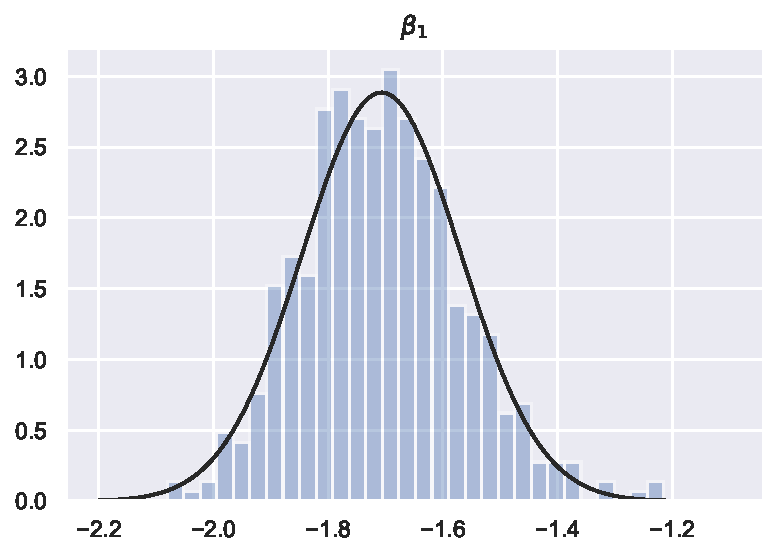
\includegraphics[width=200pt]{figures/marginal_beta_1.pdf}
		\caption{Marginal of $\beta_1$.}
		\label{fig1}
	\end{figure}
	
	
	\begin{figure}[H]
		\centering
		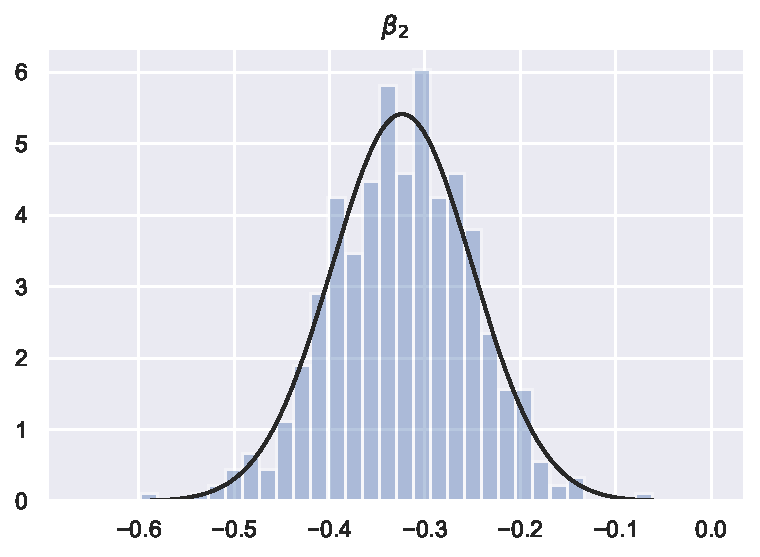
\includegraphics[width=200pt]{figures/marginal_beta_2.pdf}
		\caption{Marginal of $\beta_2$.}
		\label{fig2}
	\end{figure}


\item Make a scatter plot of $\beta_1^k$ vs $\beta_2^k$. Plot the principal directions of the actual data $X$ and the principal directions of $\beta^k$s. \\
\medskip


	\begin{figure}[H]
		\centering
		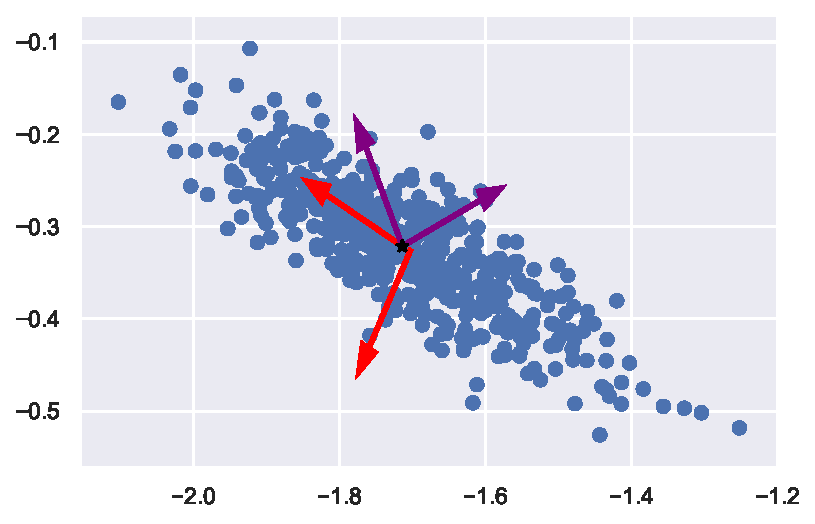
\includegraphics[width=200pt]{figures/scatter_plot.pdf}
		\caption{The two principal directions of $X$ are along the two red arrows while the two principal directions of the cloud of $\beta$ coefficients are along the purple arrows.}
		\label{fig3}
	\end{figure}
	
\item Do the principal directions of $X$ datapoints and $\beta^k$ datapoints align? Give a condition on the data generation process under which these principal directions will align. \\

\medskip
The principal directions of $X$ datapoints and $\beta^k$ datapoints do not align (even when running different samplings of the bootstrap process). 
The principal directions align when the cloud of $\beta$ coefficients is distributed along the principal directions of the datapoints $X$. The principal directions align when,
like proved in theorem 4.3 of the linear regression notes, the covariance of the $\beta$ coefficients is $\sigma^2 U S^{-2} U^T$ where SVD of $X$ is $U S V^T$.

 	\begin{figure}[H]
		\centering
		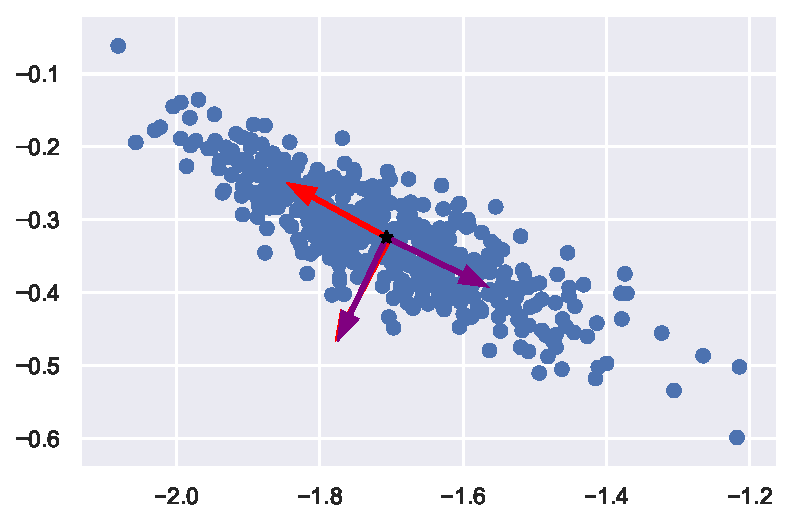
\includegraphics[width=200pt]{figures/scatter_plot_2.pdf}
		\caption{The two principal directions of $X$ are aligned with the two principal directions of the cloud of $\beta$ coefficients.}
		\label{fig3}
	\end{figure}

\end{enumerate}
\end{enumerate}
\end{document}
